%%%% fs-run-time-data-flow  FlameStream data flow

\label {fs-data-flow}

\subsection{Stream}

The top level of our data flow abstraction is a {\it stream}. Stream is represented by an ordered unlimited sequence of data items. Data item is a {\it payload} and a {\it meta-data} associated with it. Payload is an arbitrary user-provided data. Meta-data is a structured system-assigned information. The primary purpose of the meta-data is to impose the total order on data items. 

\[DataItem := (payload, Meta)\]

Data payloads are got in stream through {\it front} and got out through {\it barrier}. Particularly, front creates data items from input payloads by assigning them meta-data. Inside stream, data items can be dropped or their payloads and metas can be transformed. Eventually, barrier removes meta-information and outputs back pure payloads. The concept of the stream is shown on the figure <>.

\subsection{Graph}

In our model, the stream between front and barrier is handled by a directed data flow graph. Each node of the graph contains single operation, also called job or procedure, which can have multiple inputs and outputs. Edges show the order of these operations. The data items are processed one-by-one in a "streaming" manner.

Notably, despite the fact that commonly dataflow graphs assumed to be acyclic (DAGs) 
~\cite{Zaharia:2016:ASU:3013530.2934664, Carbone:2017:SMA:3137765.3137777},
our model does not have this restriction. Moreover, as we show further in this section, there are cases when cycles are required, e.g. for MapReduce-based algorithms. 

\subsection{Physical deployment and partitioning}

Each computational unit in our distributed runtime runs process called {\it worker}, and each worker executes complete data flow graph. Every worker is assigned by an integer interval. Intervals are not intersected and cover the range of 32-bit signed integer.

Each input of each operation is assigned by user-provided hash function called {\it balancing function}. This function is applied to the payload of data items and determines partitioning. More precisely, its value is computed each time before the next operation. After that, corresponding data item is sent to the worker, which is responsible for the computed value. Therefore, load balancing explicitly depends on the balancing functions of the operations. The balancing functions are the part of business logic, because optimal balancing requires the knowledge of payload distribution.

Figure~\ref{logical-graph-figure} shows the example of data flow graph. Possible partitioning of this graph on two nodes is shown on the figure~\ref{physical-graph-figure}.

\begin{figure}[htbp]
  \centering
  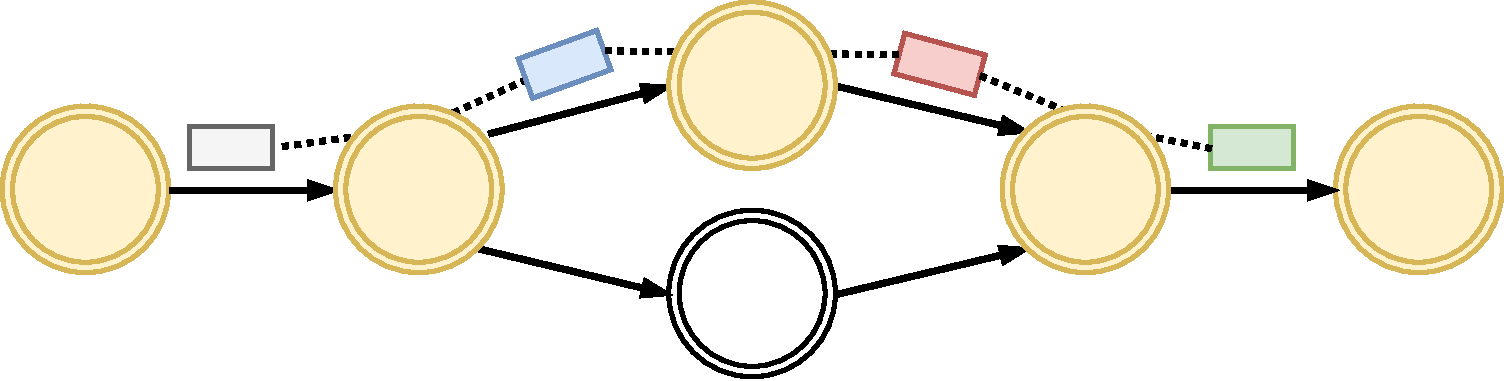
\includegraphics[width=0.48\textwidth]{pics/logical-graph}
  \caption{The example of data flow graph}
  \label {logical-graph-figure}
\end{figure}

\begin{figure}[htbp]
  \centering
  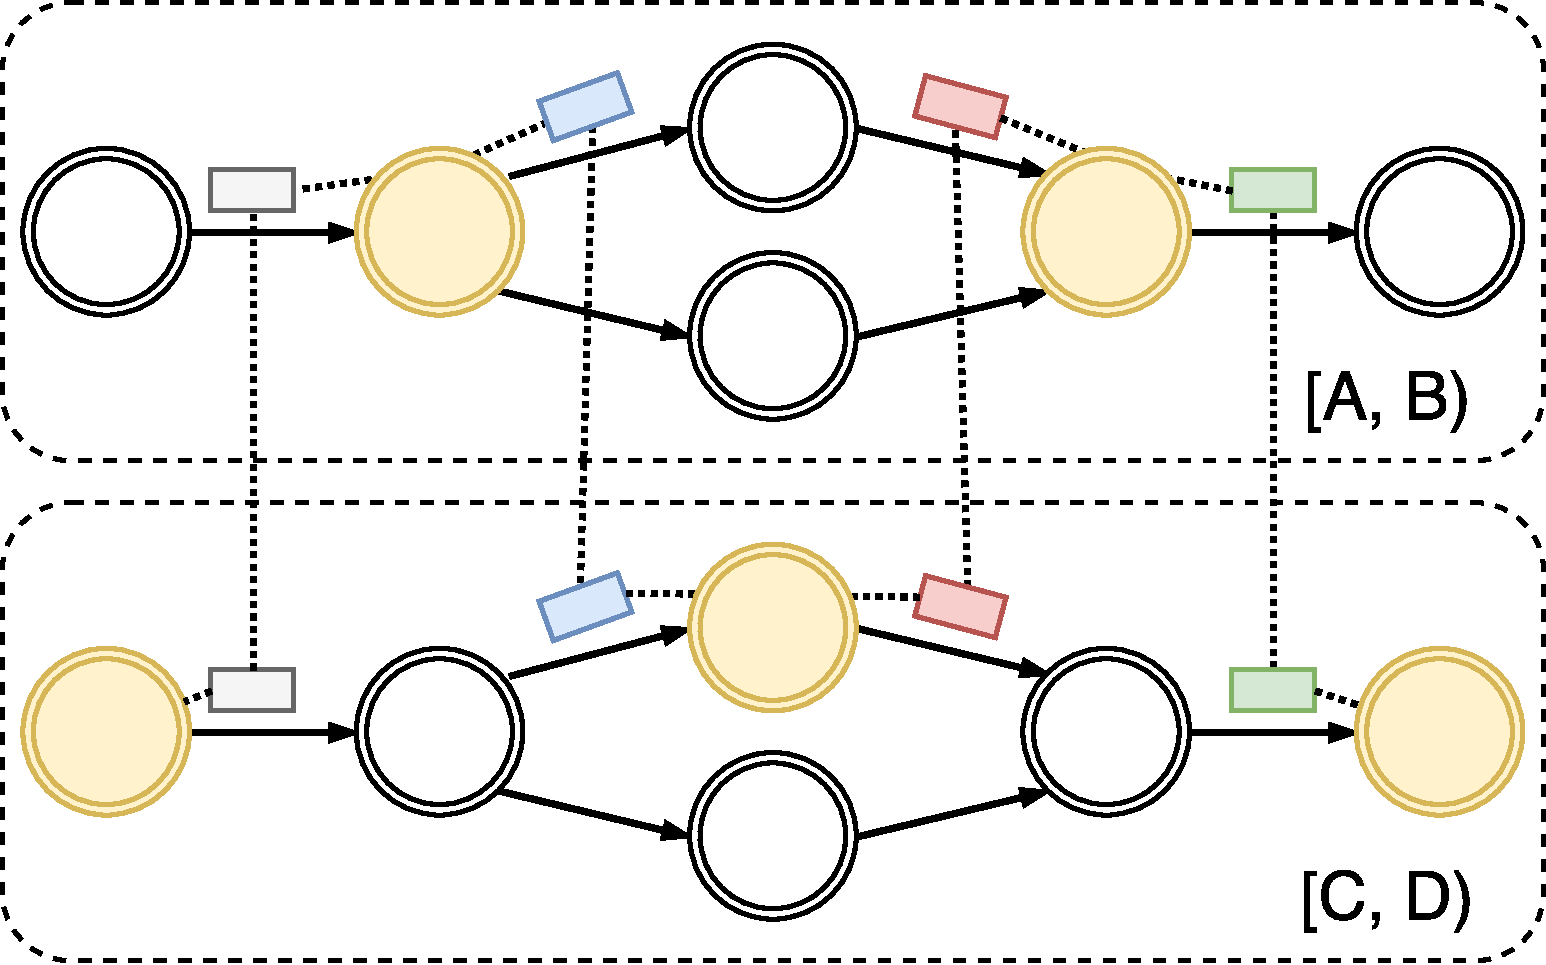
\includegraphics[width=0.48\textwidth]{pics/physical-graph}
  \caption{Possible partitioning of the data flow graph}
  \label {physical-graph-figure}
\end{figure}

\subsection{Ordering model}

As it was mentioned above, meta-information imposes explicit total order on data items. Without diving into the details, it should be noted that the order of items is maintained across different fronts.

Let {\it image} is an output data item of an operation and {\it preimage} is a corresponding input item. In this terms, the order of images is preserved, i.e. the order of images is the same as the order of preimages. Moreover, the image of the item is greater than its preimage but less than the next item. The concept of ordering is shown on the figure <>.

We assume that input items of the operations are strictly ordered. The approach for satisfying such ordering properties is detailed in the following sections.

It is worth to mention, that after the meta-data is assigned to data item at the front, the rest of computations become deterministic.

\subsection{Operations}

The set of available operations is limited by the following list.

{\bf Map} applies user-defined transformation to the payload of input item. 

{\bf Flat map} applies user-defined function to the payload of input item. This function returns a sequence of new payloads. Each of these payloads is put into distinct data item. 

{\bf Filter} applies user-defined predicate to the payload of input item. If the result of predicate is positive, filter outputs initial item with updated trace of local times. Otherwise, filter outputs nothing.

{\bf Broadcast} replicates input item to the specified number of operations or sinks. 

{\bf Merge} operation is initialized with specified number of input nodes. Each input item from all input nodes is sent to the single output. It preserves ordering between input items.

{\bf Grouping} has two parameters: number called {\it window} and hash function. Grouping stores input items in distinct buckets by the value of the hash function applied to payload. When next in turn item is got in the grouping, it is put to the tail of corresponding bucket. After that, grouping outputs window-sized {\it tuple item}, which consists of the last items of this bucket. If the size of bucket is less than window, all items of bucket are taken. Notably, grouping is the only operation that maintains state.
	
We assume that hash functions in grouping are perfect, i.e. do not have any collisions. However, practically, user can define equivalence relation to ensure that items with distinct payloads are got in the distinct buffers.
	
To completely clarify the semantics of this operation, consider the following example. The grouping accepts items with payload represented as natural numbers: 1,2,3, etc. The hash function returns 1 if the number is even and 0 otherwise. If the window is set to 3, the output is:

\[(1), (2), (1|3), (2|4), (1|3|5), (2|4|6), (3|5|7), (4|6|8)...\]

The data items within tuple are ordered by the meta-information. 

The important property of the grouping is that the result is uniquely determined by the last element in the tuple. Therefore, grouping is the bijective mapping. Additionally, the results among items with different values of hash function are independent.

\subsection{User-defined parameters}

Regarding the model that we introduced in the previous sections, user can set up the following parameters:

\begin{enumerate}
  \item{Map function}
  \item{Flat map function}
  \item{Filter predicate}
  \item{Grouping window}
  \item{Balancing functions of the inputs}
  \item{Graph itself: vertices and edges}
\end{enumerate}

Grouping hash function is inherited from its balancing function. It provides independence between graph and its physical execution. 

It is important to mention, that there are no parameters for state-management. Therefore, business-logic is stateless. Nevertheless, it is enough to implement any MapReduce transformation, that is shown in the next section.

Notably, the list of parameters is quite short. Conceptually, it means that there can be a lot of data flow graphs, which can produce equivalent results. This property is useful for the graph optimization problem.    


